\documentclass[conference,letterpaper]{IEEEtran}\IEEEoverridecommandlockouts

\usepackage{graphicx}
\usepackage{amsmath,amssymb}
\usepackage{newtxtext,newtxmath}
\usepackage{booktabs}
\usepackage{array}
\usepackage{tabularx}
\usepackage{makecell}
\usepackage{multirow}
\usepackage{url}
\usepackage{xcolor}
\usepackage{cite}
\usepackage{stfloats}
\usepackage{placeins}
\usepackage{balance}
\usepackage{flushend}
\usepackage{caption}
\captionsetup[figure]{font=footnotesize,skip=2pt}
\captionsetup[table]{font=footnotesize,skip=2pt}

% Template-style footer adapted from the PHM-Ji'nan 2026 Word template.
% The official Word template uses US-letter two-column layout, Times-style fonts,
% unnumbered pages, and a conference footer at the bottom of each page.
\usepackage{fancyhdr}
\setlength{\headheight}{12pt}
\setlength{\footskip}{27pt}
\fancypagestyle{phmregular}{%
  \fancyhf{}%
  \fancyfoot[R]{\scriptsize 2026 Global Reliability and Prognostics and Health Management\\[-1pt](PHM-Ji'nan)}%
  \renewcommand{\headrulewidth}{0pt}%
  \renewcommand{\footrulewidth}{0pt}%
}
\fancypagestyle{phmfirst}{%
  \fancyhf{}%
  \fancyfoot[L]{\scriptsize \begin{tabular}{@{}l@{}}\rule{0.43\columnwidth}{0.4pt}\\[-1pt]Supported by Grant No. 2025-JKZK-HZ-14.\end{tabular}}%
  \fancyfoot[R]{\scriptsize 2026 Global Reliability and Prognostics and Health Management\\[-1pt](PHM-Ji'nan)}%
  \renewcommand{\headrulewidth}{0pt}%
  \renewcommand{\footrulewidth}{0pt}%
}

\newcolumntype{L}[1]{>{\raggedright\arraybackslash}p{#1}}
\newcolumntype{C}[1]{>{\centering\arraybackslash}p{#1}}
\newcolumntype{Y}{>{\raggedright\arraybackslash}X}
\renewcommand{\arraystretch}{1.05}

\newcommand{\algorule}{\noindent\rule{\linewidth}{0.6pt}}
\newenvironment{algorithmblock}[1]{%
    \begin{minipage}{0.98\linewidth}
    \algorule\vspace{2pt}
    {\small\textbf{#1}}\par\vspace{2pt}
    \algorule\vspace{2pt}
    \footnotesize
}{%
    \vspace{2pt}\algorule
    \end{minipage}
}

\title{Anti-Forgetting Transfer Learning for Cross-Condition PMSM Stator Fault Diagnosis with Time-Frequency CrossViT}

\author{%
\begin{tabular*}{\textwidth}{@{\extracolsep{\fill}}cc@{}}
\begin{minipage}{0.45\textwidth}\centering
\normalsize Shilang Huang\\[-0.15ex]
\small Department of Industrial Engineering\\
\small Tsinghua University\\
\small Beijing 100084, China\\
\small huangsl23@mails.tsinghua.edu.cn
\end{minipage} &
\begin{minipage}{0.45\textwidth}\centering
\normalsize Zhenning Li\\[-0.15ex]
\small Department of Industrial Engineering\\
\small Tsinghua University\\
\small Beijing 100084, China\\
\small lizhenning@mail.tsinghua.edu.cn
\end{minipage}\\[3.0em]
\begin{minipage}{0.45\textwidth}\centering
\normalsize Ruiguan Lin\\[-0.15ex]
\small Department of Industrial Engineering\\
\small Tsinghua University\\
\small Beijing 100084, China\\
\small linruiguan@nuaa.edu.cn
\end{minipage} &
\begin{minipage}{0.45\textwidth}\centering
\normalsize Ai He\\[-0.15ex]
\small Institute for Aero Engine\\
\small Tsinghua University\\
\small Beijing 100084, China\\
\small heai@mails.tsinghua.edu.cn
\end{minipage}
\end{tabular*}%
}

\begin{document}
\maketitle
\thispagestyle{phmfirst}
\pagestyle{phmregular}

\begin{abstract}
Fault diagnosis models in prognostics and health management (PHM) often face cross-condition distribution shifts, because the same type of motor may operate under different rated capacities or load-related environments. Transfer learning is a natural solution, but direct target-domain fine-tuning can cause catastrophic forgetting and degrade the model's ability to recognize source-domain faults. This paper studies this problem on a cross-capacity permanent-magnet synchronous motor (PMSM) stator-fault diagnosis task. A time-frequency CrossViT backbone is used to fuse time-domain vibration windows and STFT spectrograms, and an anti-forgetting transfer pipeline is built with teacher-student distillation, LWF-style replay, optional freezing, and EWC regularization. Experiments show that the proposed anti-forgetting transfer strategy achieves effective target adaptation while better preserving source-domain knowledge, demonstrating robust overall performance across different capacities.
\end{abstract}

\begin{IEEEkeywords}
PMSM fault diagnosis, cross-condition transfer, time-frequency CrossViT, catastrophic forgetting, knowledge distillation, PHM.
\end{IEEEkeywords}


\section{Introduction}
Electric motors are key components in manufacturing equipment, transportation systems, and energy conversion devices. Unexpected stator or winding faults may cause efficiency degradation, unplanned downtime, and safety risks. PHM techniques therefore require reliable fault diagnosis models that can identify fault patterns under changing operating conditions. Deep learning has become an effective tool for this purpose because it can learn discriminative representations from high-dimensional time-series measurements and time-frequency images. Recent PHM and industrial monitoring studies further show that deep models and foundation-model-style visual reasoning can improve health assessment and industrial inspection under complex scenarios \cite{zhang2022review,wang2024defectglm}.

In practical motor systems, however, the training and deployment domains are often not identical. A model calibrated on one capacity or load-related condition may face shifted amplitude distributions, frequency components, and time-frequency structures when it is transferred to another condition. This work therefore describes the task as cross-condition or cross-capacity fault diagnosis rather than cross-capacity diagnosis, avoiding confusion with the signal-processing term cross-capacity spectrum. Existing transfer diagnosis and domain adaptation methods attempt to reduce such distribution discrepancy and improve target-domain recognition \cite{cao2021dscnn,yang2018can,du2019hybrid,xing2023dsfan,guan2025ucmg}.

A limitation of many transfer diagnosis studies is that target-domain accuracy is treated as the dominant goal, while source-domain knowledge retention is rarely evaluated. In industrial PHM, a diagnostic system may be reused across multiple motors or repeatedly switch among working conditions. If direct fine-tuning adapts the model to a new target domain but destroys the source decision boundary, the resulting model becomes unreliable for multi-condition deployment. This is a catastrophic forgetting problem in a transfer-learning context.

To address this issue, this paper formulates cross-capacity PMSM stator fault diagnosis as a dual-objective transfer problem: the model should adapt to the target capacity while preserving source-domain fault knowledge. Methodologically, the proposed pipeline combines a time-frequency CrossViT backbone with anti-forgetting strategies from continual learning. The backbone extracts local temporal patterns from the vibration branch, spectral and time-frequency structures from the spectrogram branch, and complementary diagnostic cues through attention-based multi-modal fusion. The transfer stage is designed as an anti-forgetting pipeline: a source-domain teacher constrains the student with softened decision distributions, replayed source windows stabilize old decision boundaries, and optional freezing or EWC limits destructive parameter drift.

The main methodological contributions are summarized as follows. First, we construct a time-frequency CrossViT diagnostic model tailored to cross-condition PMSM stator-fault diagnosis, so that waveform-level transients and spectrogram-level fault signatures can be represented in a unified framework. Second, we design a transfer pipeline with explicit anti-forgetting ability, in which teacher-student distillation and LWF-style replay jointly maintain source-domain decision structure during target adaptation. Beyond these two method components, the paper reports a systematic ablation from basic fine-tuning to domain adaptation and continual-learning variants, demonstrating when target adaptation and source retention become compatible or conflicting.

\section{Related Work}
\subsection{Deep Learning and Multi-Modal Fault Diagnosis}
Deep learning-based fault diagnosis has been widely studied for rotating machinery. CNN-based and transformer-based models can learn local and long-range signal structures in an end-to-end manner. Time-frequency representations, such as STFT and wavelet-based maps, are also frequently used because they reveal frequency and energy distributions that may not be obvious in raw time signals. Recent work has further combined convolutional modules and attention mechanisms to extract local and global representations for bearing diagnosis \cite{yu2023adaptive}. Dual-domain signal fusion methods also indicate that time-domain and frequency-domain signals provide complementary information for cross-domain diagnosis \cite{xing2023dsfan}.

\subsection{Transfer Learning and Domain Adaptation}
Transfer learning uses source-domain knowledge to improve target-domain learning. In fault diagnosis, the source domain usually contains sufficient labeled samples, while the target domain may contain limited or unlabeled samples under another machine, load, or capacity condition. Domain adaptation methods reduce feature discrepancy between domains through distribution matching or adversarial learning. DSCNN and CAN minimize MK-MMD to learn transferable features \cite{gretton2012mmd,cao2021dscnn,yang2018can}. DANN introduces a domain discriminator and gradient reversal layer to learn domain-invariant representations \cite{ganin2016dann}. Other methods jointly align marginal and conditional distributions, or use Wasserstein distance and adversarial training to improve transfer performance \cite{long2017jan,xiao2022njtn,yu2023adaptive}.

Although these methods are effective for target-domain adaptation, they do not always preserve source-domain performance. Distribution alignment may push the representation toward domain invariance, but domain invariance alone cannot guarantee old decision-boundary retention. This motivates the use of continual-learning strategies in cross-condition diagnosis.

\subsection{Continual Learning and Knowledge Retention}
Continual learning studies how a model can learn new tasks without forgetting old ones. EWC protects important parameters by using a Fisher-information-weighted penalty \cite{kirkpatrick2017ewc}. Knowledge distillation transfers the softened output distribution of a teacher model to a student model \cite{hinton2015distill}. LWF constrains the new model to preserve old-task responses during new-task learning \cite{li2018lwf}. In this paper, these strategies are adapted to cross-capacity fault diagnosis. The source-domain model is regarded as a teacher, and source replay is used to maintain source decision boundaries while learning target-domain features.


\section{Method}
The overall framework of the proposed method is illustrated in Fig.~\ref{fig:overall_framework}. It contains four stages: multi-modal data construction, a detailed time-frequency CrossViT diagnosis backbone, source-domain pre-training, and evaluation-oriented visualization.

\begin{figure*}[!t]
\centering
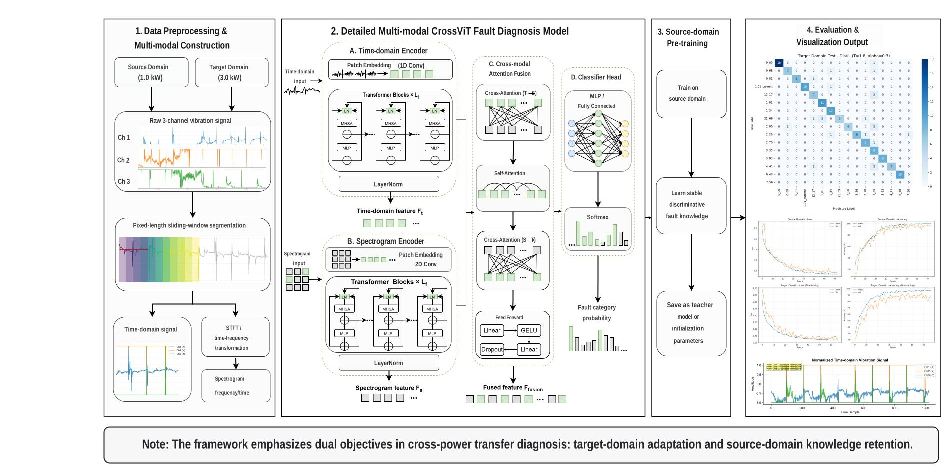
\includegraphics[width=0.95\textwidth]{figures/overall_framework_latest_cropped_clean.pdf}
\caption{Overall framework of the proposed anti-forgetting transfer diagnosis method for cross-capacity PMSM stator faults.}
\label{fig:overall_framework}
\end{figure*}


\subsection{Problem Definition and Multi-Modal Construction}
Let $D_s=\{(x_i^s,y_i^s)\}_{i=1}^{n_s}$ denote the labeled source domain collected from a 1.0 kW PMSM and $D_t=\{(x_i^t,y_i^t)\}_{i=1}^{n_t}$ denote the target domain collected from a 3.0 kW PMSM. The two domains share the same stator-fault label space, but their feature distributions differ due to motor-capacity variation, i.e., $P_s(x)\neq P_t(x)$. Each processed sample is represented as a three-channel time-series window. The window is also transformed into a time-frequency spectrogram by STFT. Thus, the input of each sample contains two complementary modalities: a time-domain signal $x_{time}$ and a spectrogram $x_{spec}$.


\subsection{Multi-Modal CrossViT Backbone}
The backbone contains a time-domain encoder, a spectrogram encoder, a cross-modal attention fusion module, and a classifier head. The time-domain encoder projects the segmented waveform into tokens and models local temporal dependencies caused by impacts and transient variations. The spectrogram encoder uses two-dimensional patch embedding and transformer blocks to capture frequency bands and time-frequency energy structures. The two encoded representations are then fused at the modality level so that temporal and spectral cues jointly determine the fault category:
\begin{equation}
F_t=E_t(x_{time}),\quad F_s=E_s(x_{spec}),
\end{equation}
\begin{equation}
F_{fusion}=A_{cross}(F_t,F_s),\quad \hat{y}=C(F_{fusion}),
\end{equation}
where $E_t$ and $E_s$ are the two encoders, $A_{cross}(\cdot)$ denotes cross-modal attention fusion, and $C(\cdot)$ is the classifier. The purpose of this architecture is not only to improve recognition accuracy, but also to provide a stable feature basis for subsequent anti-forgetting transfer.

\subsection{Source-Domain Pre-Training}
The first stage trains the multi-modal CrossViT on the source domain. The source loss is the standard cross-entropy loss:
\begin{equation}
\mathcal{L}_{src}=-\frac{1}{B}\sum_{i=1}^{B}\sum_{c=1}^{C}\mathbf{1}(y_i=c)\log p_i(c).
\end{equation}
The trained model is saved as a teacher model $f_{\theta^*}$ and also provides initialization for target adaptation. The concrete source-domain pre-training workflow is summarized in Fig.~\ref{alg:pretrain}, which is placed immediately after this subsection to make the algorithmic stage explicit.

\begin{figure}[!t]
\centering
\begin{algorithmblock}{Algorithm 1: Multi-Modal Source-Domain Pre-Training}
\textbf{Input:} source domain $D_s$, model $f_\theta$, maximum epochs $E_s$.\\
\textbf{Output:} teacher model $f_{\theta^*}$ and initialization parameters.\\[1mm]
1: Initialize time encoder, spectrogram encoder, fusion module and classifier.\\
2: \textbf{for} epoch $=1,\ldots,E_s$ \textbf{do}\\
3: \quad Sample a mini-batch $(x_{time}^s,x_{spec}^s,y^s)$ from $D_s$.\\
4: \quad Compute $F_t=E_t(x_{time}^s)$ and $F_s=E_s(x_{spec}^s)$.\\
5: \quad Fuse features by $F_{fusion}=\mathcal{A}_{cross}(F_t,F_s)$.\\
6: \quad Predict $\hat{y}^s=C(F_{fusion})$ and compute $\mathcal{L}_{src}$.\\
7: \quad Update model parameters by back-propagation.\\
8: \textbf{end for}\\
9: Save the best source-domain model as teacher $f_{\theta^*}$.
\end{algorithmblock}
\caption{Source-domain pre-training for stable fault knowledge learning.}
\label{alg:pretrain}
\end{figure}

\subsection{Anti-Forgetting Transfer With Distillation, LWF and Freezing}
During target adaptation, direct fine-tuning can overwrite source-domain representations. To reduce forgetting, the proposed strategy combines three mechanisms. First, layer freezing is optionally used to reduce large parameter drift in early encoders. Second, a teacher model provides soft labels. Third, source replay following the LWF idea mixes a small ratio of source-domain samples with target-domain samples.

The knowledge distillation loss is
\begin{equation}
\mathcal{L}_{KD}=T^2\,\mathrm{KL}\left(\sigma\left(z_s/T\right),\sigma\left(z_T/T\right)\right),
\end{equation}
where $z_s$ and $z_T$ are student and teacher logits, $T$ is the temperature, and $\sigma(\cdot)$ is softmax. The final loss is
\begin{equation}
\mathcal{L}= (1-\alpha)\mathcal{L}_{CE}+\alpha\mathcal{L}_{KD}+\lambda_e\mathcal{L}_{EWC},
\end{equation}
where $\alpha$ controls the distillation weight and $\mathcal{L}_{EWC}$ is optional. Fig.~\ref{alg:antiforgetting} gives the complete anti-forgetting transfer procedure, including layer freezing, EWC, teacher-student distillation and LWF-style replay.

\begin{figure}[!t]
\centering
\begin{algorithmblock}{Algorithm 2: Anti-Forgetting Transfer With Freezing, EWC, Distillation and LWF}
\textbf{Input:} teacher $f_{\theta^*}$, source replay set $R_s$, target set $D_t$, temperature $T$, weight $\alpha$.\\
\textbf{Output:} adapted model $f_{\theta'}$.\\[1mm]
1: Initialize student $f_\theta \leftarrow f_{\theta^*}$.\\
2: Freeze selected embedding or encoder layers if required.\\
3: Estimate Fisher matrix on $D_s$ when EWC is enabled.\\
4: \textbf{for} epoch $=1,\ldots,E_t$ \textbf{do}\\
5: \quad Sample target mini-batch $B_t$ and replay mini-batch $B_s\subset R_s$.\\
6: \quad Compute student logits $z_s$ and teacher logits $z_T$.\\
7: \quad Compute hard-label loss $\mathcal{L}_{CE}$ on available labels.\\
8: \quad Compute distillation loss $\mathcal{L}_{KD}$ from softened teacher outputs.\\
9: \quad Add optional $\mathcal{L}_{EWC}$ to protect important parameters.\\
10: \quad Optimize $\mathcal{L}=(1-\alpha)\mathcal{L}_{CE}+\alpha\mathcal{L}_{KD}+\lambda_e\mathcal{L}_{EWC}$.\\
11: \textbf{end for}\\
12: Return the model with the best Balance Score.
\end{algorithmblock}
\caption{Anti-forgetting transfer procedure used in the final recommended pipeline.}
\label{alg:antiforgetting}
\end{figure}

\subsection{Domain Adaptation Candidates and Model Selection}
DANN, MMD and pseudo-labeling are treated as ablation candidates. DANN uses a domain discriminator connected by a gradient reversal layer. MMD minimizes feature-distribution discrepancy. Pseudo-labeling selects high-confidence target predictions as temporary labels. Since these methods may improve target-domain accuracy while damaging source retention, the final model is selected by a dual-domain Balance Score:
\begin{equation}
S_{bal}=A_t-\beta \max(0,A_s^{ref}-A_s),
\end{equation}
where $A_t$ is target accuracy, $A_s$ is source accuracy, and $A_s^{ref}$ is a source retention reference. A higher $S_{bal}$ indicates a better balance. This score is not an average accuracy; it is a task-specific retention-aware criterion for model selection. Fig.~\ref{alg:selection} further shows how the candidate methods are compared and selected under the dual-domain criterion.

\begin{figure}[!t]
\centering
\begin{algorithmblock}{Algorithm 3: Ablation Candidates and Dual-Domain Model Selection}
\textbf{Input:} candidate set $\mathcal{M}$, source test set, target test set.\\
\textbf{Output:} selected model $m^*$.\\[1mm]
1: Construct candidates: fine-tuning, freezing, EWC, Distill, Distill+LWF, DANN, MMD and pseudo-labeling.\\
2: \textbf{for each} candidate $m\in\mathcal{M}$ \textbf{do}\\
3: \quad Train or adapt $m$ under the same source-target task.\\
4: \quad Evaluate source retention $A_s(m)$ and target accuracy $A_t(m)$.\\
5: \quad Compute Balance Score $S_{bal}(m)$.\\
6: \textbf{end for}\\
7: Select $m^*=\arg\max_m S_{bal}(m)$.\\
8: Generate confusion matrices, training curves and attention maps for $m^*$.
\end{algorithmblock}
\caption{Ablation-driven model selection for dual-objective transfer diagnosis.}
\label{alg:selection}
\end{figure}

\section{Experiments}

\subsection{Dataset and Experimental Settings}
The experiments use Dataset 2 in the collected dataset document, namely the KAIST/Mendeley Data PMSM stator-fault dataset \cite{jung2023data}. The public benchmark was collected on a PMSM fault-diagnosis testbed containing three-phase motors with capacities of 1.0 kW, 1.5 kW, and 3.0 kW. The motors were tested at 3000 RPM under the same load setting. The measurement system used an IEPE piezoelectric accelerometer for vibration and three current transformers for phase-current acquisition, connected to NI data-acquisition modules. Each condition was recorded for 120 s; vibration signals were sampled at 25.6 kHz and current signals at 100 kHz. The artificial stator faults include inter-turn and inter-coil short circuits with multiple severities, making the dataset suitable for evaluating capacity-related distribution shifts.

In this paper, the 1.0 kW motor is used as the source domain and the 3.0 kW motor is used as the target domain. The released data are processed into three-channel time-series windows with length 1024 and stride 128, and each window is further transformed into a $3\times128\times128$ spectrogram by STFT. The source and target domains share a 16-class diagnosis protocol constructed from the available normal and stator-fault conditions. All compared methods use the same preprocessing, data split, backbone, and evaluation pipeline to ensure that the reported differences mainly come from the transfer strategies.

\begin{table}[!t]
\caption{Dataset Settings for Cross-Capacity PMSM Fault Diagnosis}
\label{tab:dataset}
\centering
\footnotesize
\begin{tabular}{L{2.35cm} L{5.0cm}}
\toprule
Item & Description \\
\midrule
Public source & KAIST/Mendeley PMSM stator-fault dataset \\
Motor capacities & 1.0, 1.5 and 3.0 kW; this work uses 1.0 kW $\rightarrow$ 3.0 kW \\
Operating condition & 3000 RPM under the same torque-load condition \\
Original sensors & IEPE accelerometer and three current transformers with NI DAQ \\
Original sampling & 25.6 kHz vibration, 100 kHz current, 120 s per condition \\
Processed input & $1024\times3$ time-series window and $3\times128\times128$ spectrogram \\
Fault protocol & 16-class stator-fault diagnosis setting \\
\bottomrule
\end{tabular}
\end{table}

\subsection{Overall Quantitative Results}
Table~\ref{tab:main_results} summarizes the complete experimental evolution. The observation column has been removed to keep the configuration field readable. The results include both the early baseline series and the latest updated preprocessing series. EXP1 gives the single-domain baseline. EXP2 verifies that direct cross-capacity generalization fails. EXP3 V1 to V4 then gradually introduce fine-tuning, model scaling, freezing, continual-learning strategies, and domain adaptation candidates. The slash-separated values in EXP1 and EXP2 are not repeated trials under the same pipeline. The left value corresponds to the updated dense-window protocol used in the latest experiments, i.e., a smaller stride setting with a 7:2:1 train/test/validation split; the right value corresponds to the earlier baseline protocol, which used the original preprocessing and data split. For example, in EXP1, 87.82\% is the updated dense-window baseline, whereas 90.00\% is the earlier single-domain baseline. Similarly, in EXP2, 94.23\%/4.49\% are the updated source/target results, while 85.00\%/10.00\% are the earlier source/target results. The Balance Score is a retention-aware model-selection score defined by (1), not the arithmetic mean of source and target accuracies; it is used to emphasize the joint requirement of target adaptation and source-domain retention.

\begin{table*}[!t]
\caption{Evolution of EXP1, EXP2, EXP3 V1--V4 and Latest Updated Results}
\label{tab:main_results}
\centering
\footnotesize
\setlength{\tabcolsep}{2.2pt}
\renewcommand{\arraystretch}{1.18}
\begin{tabular*}{0.90\textwidth}{@{\extracolsep{\fill}}C{1.55cm} L{4.75cm} C{1.95cm} C{1.95cm} C{2.35cm}@{}}
\toprule
Stage & Setting / Best configuration & Source (\%) & Target (\%) & \mbox{Balance Score} \\
\midrule
EXP1 & 1.0 kW single-domain baseline & 87.82 / 90.00 & -- & -- \\
EXP2 & 1.0 kW $\rightarrow$ 3.0 kW, no adaptation & 94.23 / 85.00 & 4.49 / 10.00 & -- \\
EXP3 V1 & Basic fine-tuning & 12.50 & 27.50 & 27.50 \\
EXP3 V2 & Model scaling + freezing & 5.00 & 67.50 & 67.50 \\
EXP3 V3 & Distill+LWF, $T=2$, $\alpha=0.3$ & 77.50 & 65.00 & 75.00 \\
EXP3 V4 & Distill, $T=1.8$, $\alpha=0.3$ & 60.00 & 70.00 & 80.00 \\
Latest V3 & Distill+LWF, $T=2$, $\alpha=0.3$ & 91.03 & 89.10 & 99.10 \\
Latest V4 & Distill, $T=1.5$, $\alpha=0.25$ & 94.23 & 87.18 & 97.18 \\
\bottomrule
\end{tabular*}
\end{table*}

The progression in Table~\ref{tab:main_results} shows that a naive cross-capacity model is not reliable. EXP2 obtains high source-domain accuracy but almost fails in the target domain. V1 confirms that basic fine-tuning is not sufficient. V2 improves target-domain performance through model scaling and freezing, yet source-domain retention remains very low, indicating severe catastrophic forgetting.

The V3 and V4 results further show the difference between target-oriented adaptation and anti-forgetting adaptation. Direct fine-tuning and domain-alignment candidates such as DANN and MMD can raise target-domain accuracy, but they often damage the source-domain decision boundary. EWC and simple freezing are more conservative, but they restrict target-domain adaptation and therefore do not provide the best overall trade-off.

The strongest finding is that knowledge distillation combined with LWF-style source replay gives the most stable dual-domain behavior. In the latest stride-128 setting, Distill+LWF with $T=2$ and $\alpha=0.3$ achieves 91.03\% source accuracy, 89.10\% target accuracy, and a Balance Score of 99.10. The latest V4 distillation setting with $T=1.5$ and $\alpha=0.25$ obtains the highest source retention, 94.23\%, while still maintaining 87.18\% target accuracy. Therefore, Table~\ref{tab:main_results} is sufficient to support the main quantitative conclusion, and detailed ablation results are discussed in text rather than using another dense table.

More specifically, freezing only early layers protects a small part of the representation but restricts the feature shift required by the target capacity condition. EWC introduces a Fisher-weighted constraint on important parameters, yet its performance is sensitive to the regularization weight and does not consistently prevent forgetting. DANN and MMD are useful as target-oriented domain adaptation candidates, but their low source-domain retention indicates that domain invariance alone is not equivalent to continual reliability. Pseudo-label learning is the least stable strategy in this task because the initial target predictions are not confident enough under the large capacity-induced distribution gap.

For this reason, the paper treats DANN, MMD and pseudo-label learning as ablation candidates rather than the final recommended solution. The final recommendation is a distillation-and-replay strategy: the teacher model preserves the source-domain soft decision structure, while replayed source windows prevent the classifier head from drifting completely toward the target domain.

\subsection{Visualization Analysis}
The following figures are placed after the quantitative discussion rather than immediately after the tables. This separates numerical comparison from visual evidence. The confusion matrices highlight class-level source retention and target adaptation, while the training curves show the convergence behavior of the selected distillation configurations. In addition, an encoder self-attention map is visualized for a representative correctly classified sample. Since the implemented cross-modal fusion operates after global feature pooling, post-pooling cross-attention weights describe modality-level fusion rather than token-level localization. Therefore, the attention analysis focuses on the self-attention maps inside the time-domain and spectrogram encoders, where token-level temporal and spectral dependencies are explicitly modeled.

\begin{figure}[!t]
\centering
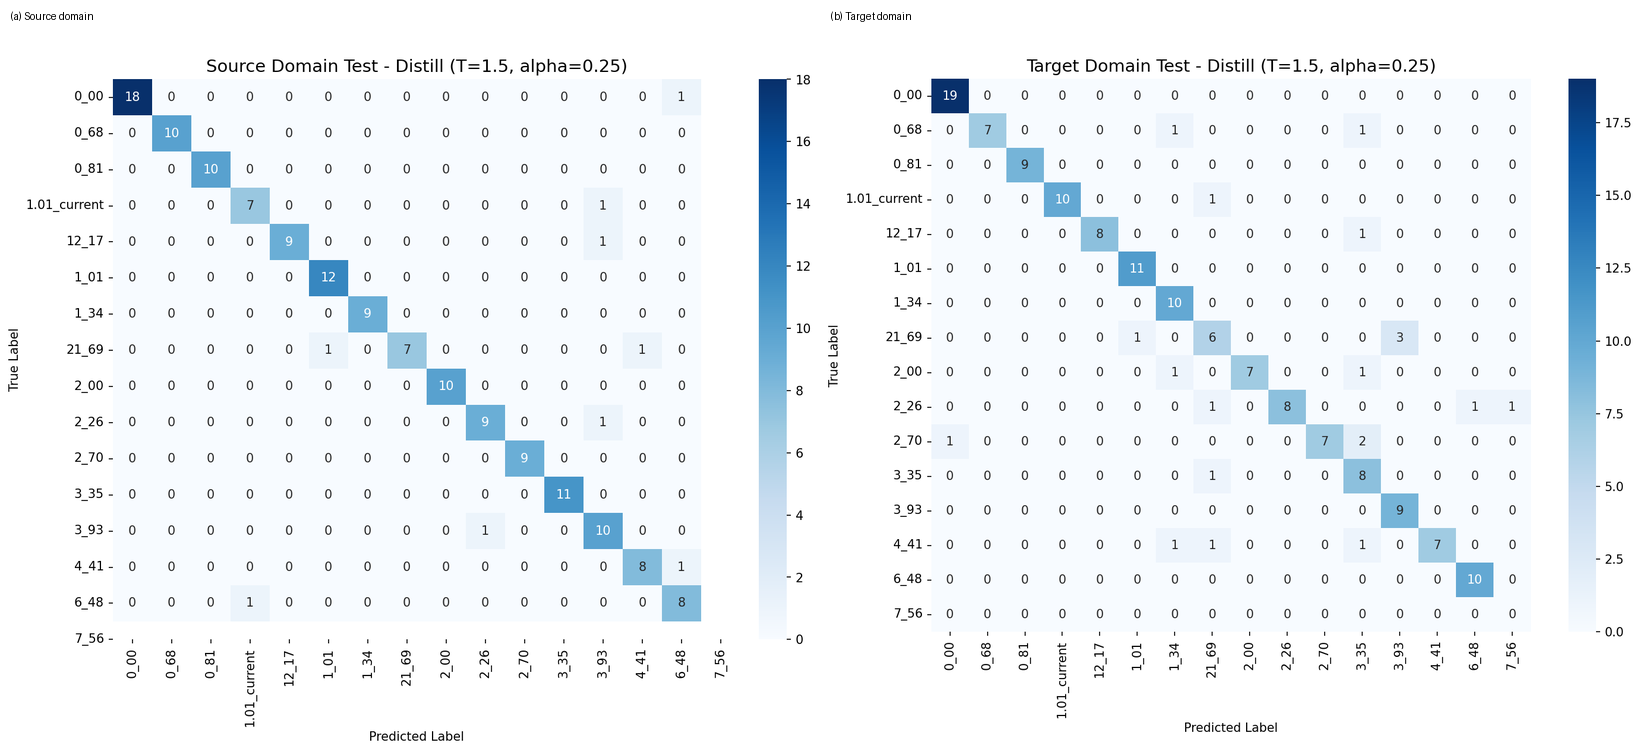
\includegraphics[width=0.98\columnwidth]{figures/fig_top1_confusions.png}
\caption{Source-domain and target-domain confusion matrices of Distill ($T=1.5$, $\alpha=0.25$).}
\label{fig:conf_v4}
\end{figure}

Fig.~\ref{fig:conf_v4} corresponds to the latest V4 configuration. The two matrices show that the model keeps a clear diagonal structure in both domains, which means the distillation objective does not simply overfit the target domain.

\begin{figure}[!t]
\centering
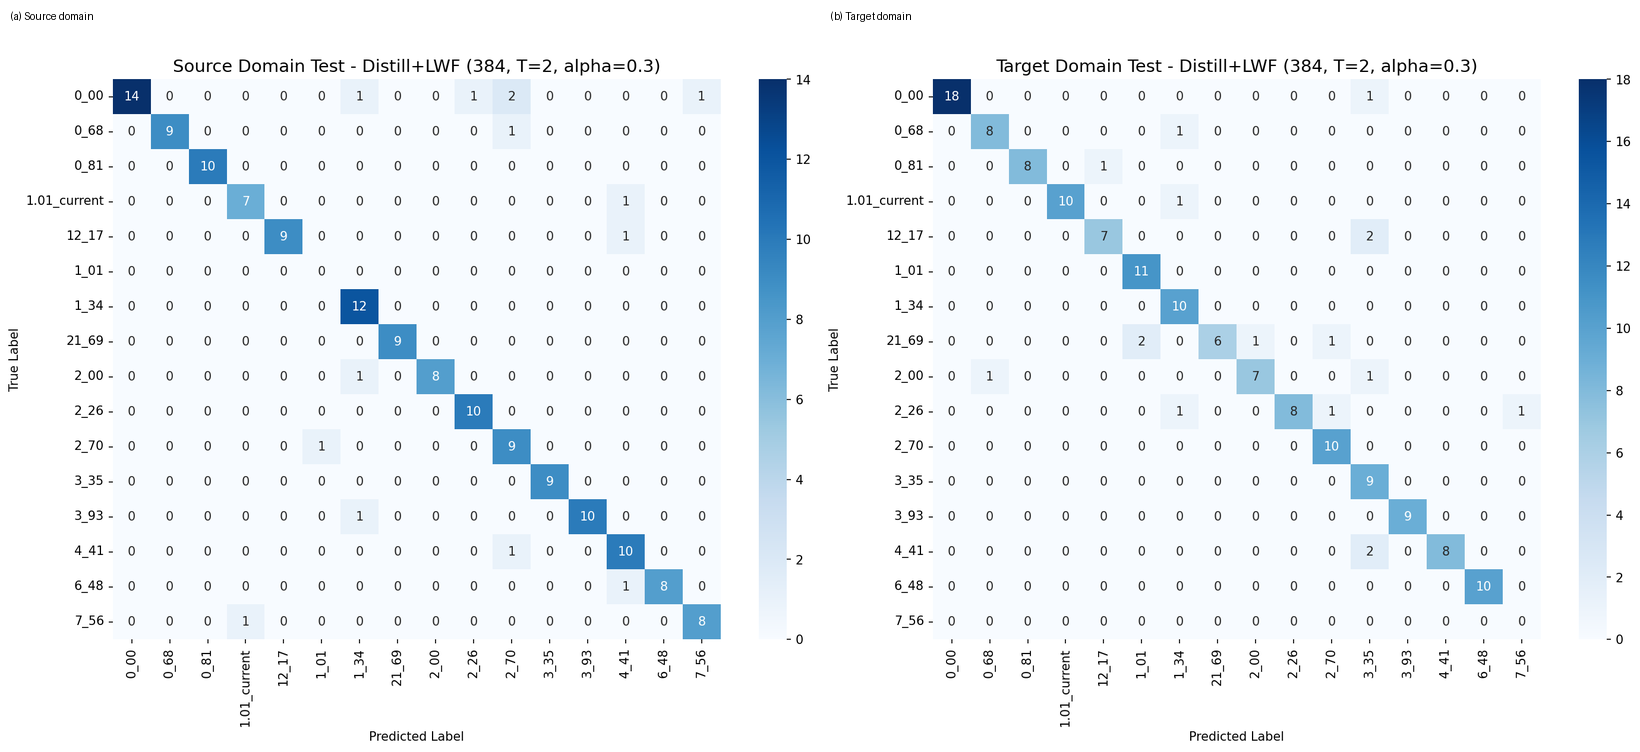
\includegraphics[width=0.98\columnwidth]{figures/fig_top2_confusions.png}
\caption{Source-domain and target-domain confusion matrices of Distill+LWF ($T=2$, $\alpha=0.3$).}
\label{fig:conf_v3}
\end{figure}

Fig.~\ref{fig:conf_v3} corresponds to the latest V3 Distill+LWF configuration, which obtains the highest Balance Score. Compared with target-only adaptation, the source-domain confusion matrix remains much more diagonal, demonstrating the effect of replay and teacher constraints. The target-domain matrix also keeps most samples around the diagonal, indicating that anti-forgetting does not simply sacrifice adaptation for retention.

\begin{figure}[!t]
\centering
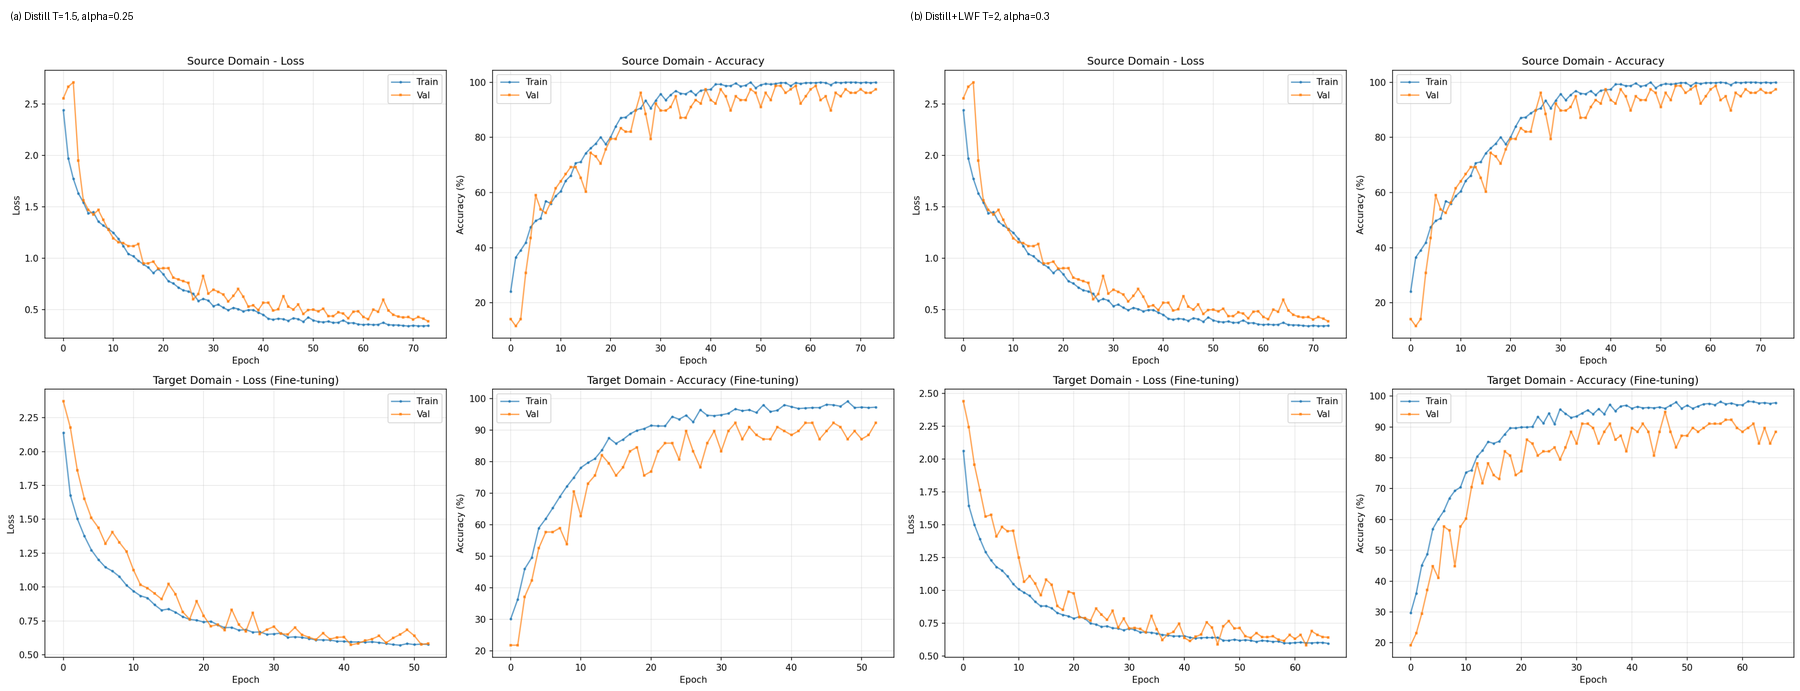
\includegraphics[width=0.98\columnwidth]{figures/fig_training_curves.png}
\caption{Training curves of representative distillation-based configurations.}
\label{fig:curves}
\end{figure}

Fig.~\ref{fig:curves} shows stable convergence during both source pre-training and target fine-tuning. The gap between training and validation accuracy is moderate in the distillation-based settings, indicating that the teacher constraint and replay samples help stabilize adaptation.

\begin{figure*}[!t]
\centering
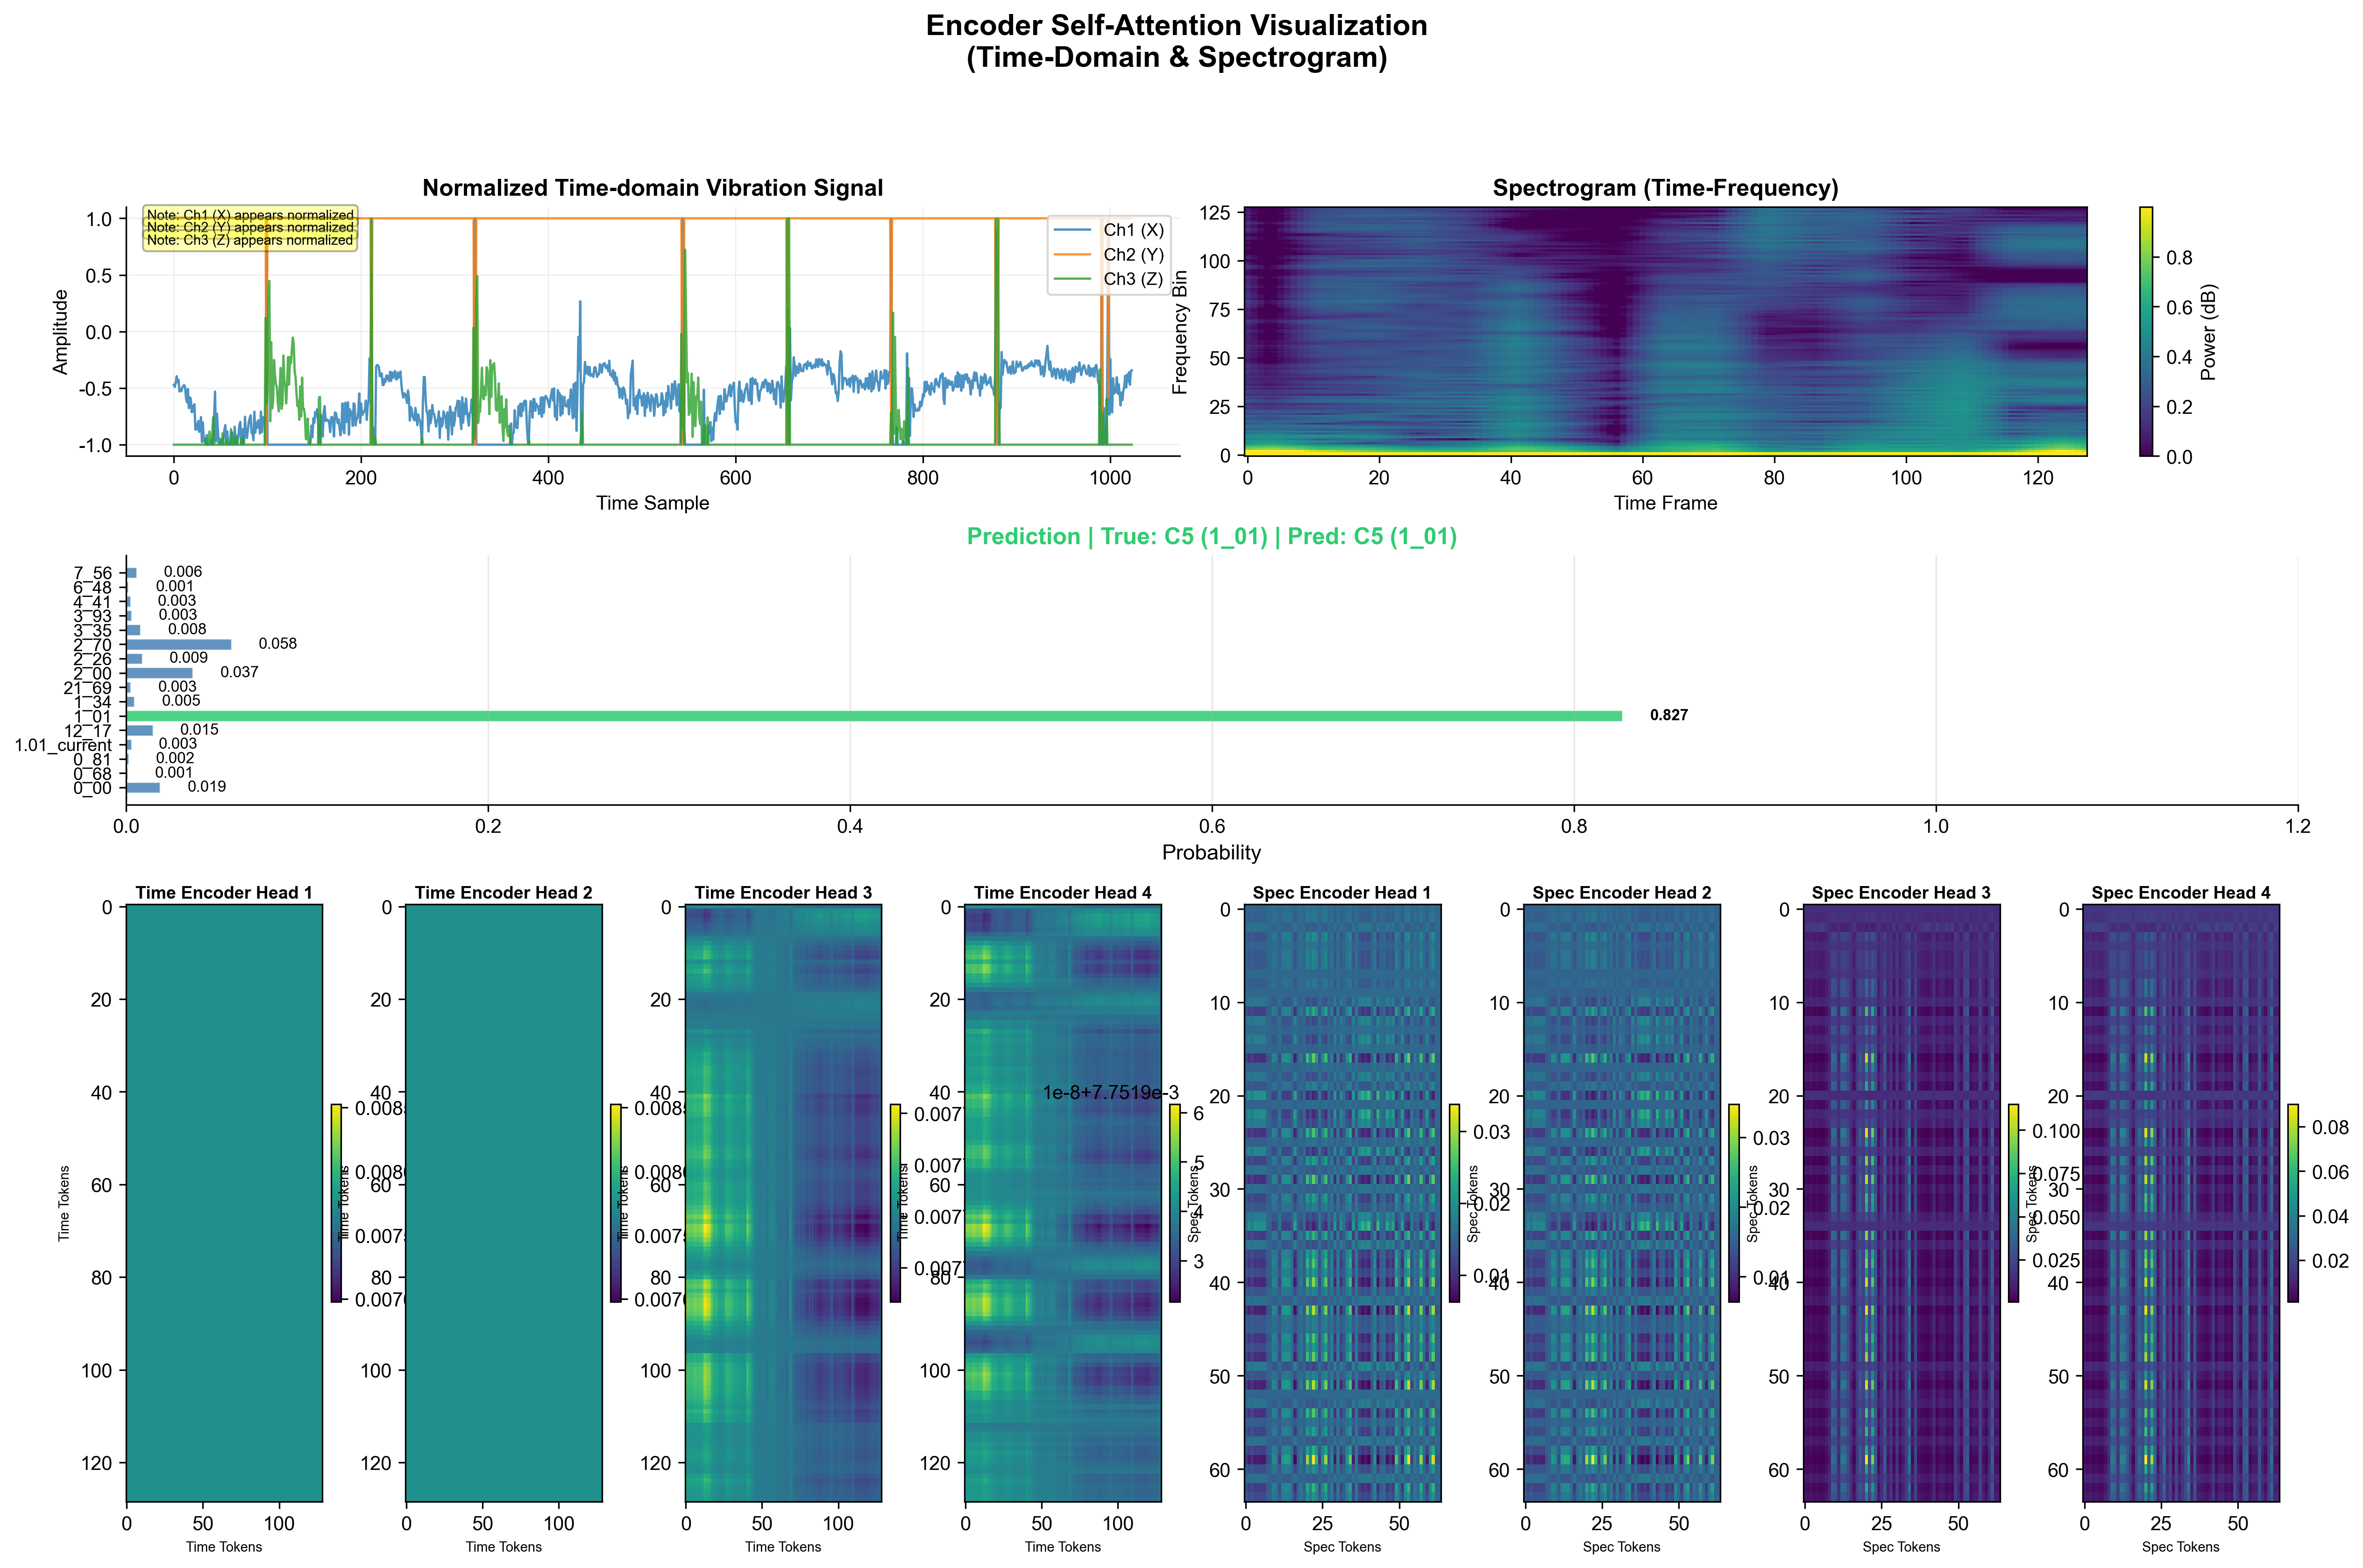
\includegraphics[width=0.88\textwidth]{figures/self_attn_correct_c5.png}
\caption{Encoder self-attention visualization for a correctly classified C5 sample. The upper part shows the normalized three-channel vibration signal, spectrogram and prediction probability, while the lower part visualizes representative self-attention heads from the time-domain and spectrogram encoders.}
\label{fig:selfattn_c5}
\end{figure*}

Fig.~\ref{fig:selfattn_c5} shows a high-confidence correctly classified C5 target-domain sample. The time-domain attention heads contain localized and banded structures, indicating that the model captures dependencies among neighboring signal patches. The spectrogram attention heads exhibit structured vertical or block-like responses over selected spectral tokens, suggesting that the frequency branch emphasizes discriminative time-frequency regions rather than uniformly attending to the whole spectrogram.


\section{Conclusion}
This paper studies cross-capacity PMSM stator fault diagnosis from the perspective of anti-forgetting transfer learning. Instead of optimizing target-domain accuracy alone, the task is formulated as a dual-objective problem that jointly evaluates target adaptation and source-domain retention. The proposed pipeline combines a time-frequency CrossViT backbone with layer freezing, EWC, teacher-student distillation, and LWF-style source replay. Experiments from EXP1 to EXP3 V4 show that pure fine-tuning and target-oriented domain adaptation candidates can improve target performance but often cause severe source-domain forgetting. In contrast, the Distill+LWF strategy provides the most stable balance. In the latest stride-128 setting, it achieves 91.03\% source accuracy, 89.10\% target accuracy, and a Balance Score of 99.10.

Future work will extend the current two-domain setting to multi-capacity and multi-source continual transfer, where the model must incrementally absorb several motor domains without repeated full retraining. Another direction is to reduce dependence on target labels through semi-supervised, open-set, or test-time adaptation, while maintaining explicit source-domain retention constraints. More practical deployment also requires online change detection, uncertainty estimation, and memory-budget control, because PHM systems may face unknown faults and limited replay storage. Finally, combining the proposed anti-forgetting pipeline with physics-informed motor indicators may further improve reliability and interpretability for real-time industrial deployment.

\FloatBarrier
\section*{Acknowledgment}
This work was supported by the Independent Scientific Research Project of Intelligent Control Laboratory (Grant No. 2025-JKZK-HZ-14). The authors used ChatGPT for language polishing, formatting assistance, and LaTeX organization; all technical claims, experimental results, and final content were checked and controlled by the authors.

% References are placed immediately after the acknowledgment without starting a new page.
\begin{thebibliography}{00}
\bibitem{zhang2022review} Y. Zhang and Y.-F. Li, ``Prognostics and health management of lithium-ion battery using deep learning methods: A review,'' \emph{Renewable and Sustainable Energy Reviews}, vol. 161, Art. no. 112282, 2022.
\bibitem{wang2024defectglm} H. Wang, C. Li, and Y.-F. Li, ``Large-scale visual language model boosted by contrast domain adaptation for intelligent industrial visual monitoring,'' \emph{IEEE Transactions on Industrial Informatics}, vol. 20, no. 12, pp. 14114--14123, 2024, doi: 10.1109/TII.2024.3441638.
\bibitem{cao2021dscnn} H. Cao, W. Luo, H. Shao, F. Zhu, M. Xia, and D. Su, ``Unsupervised domain-shared convolutional neural network for bearing fault transfer diagnosis,'' in \emph{Proc. ICCSE}, 2021, pp. 216--221.
\bibitem{yang2018can} B. Yang, Y. Lei, F. Jia, and S. Xing, ``A transfer learning method for intelligent fault diagnosis from laboratory machines to real-case machines,'' in \emph{Proc. SDPC}, 2018, pp. 35--40.
\bibitem{du2019hybrid} Z. Du, B. Yang, Y. Lei, X. Li, and N. Li, ``A hybrid transfer learning method for intelligent fault diagnosis of machinery under variable operating conditions,'' in \emph{Proc. PHM-Qingdao}, 2019.
\bibitem{xing2023dsfan} S. Xing, J. Wang, B. Han, Z. Zhang, X. Jiang, H. Ma, X. Zhang, and H. Shao, ``Dual-domain signal fusion adversarial network based Vision Transformer for cross-domain fault diagnosis,'' in \emph{Proc. PHM-Hangzhou}, 2023.
\bibitem{guan2025ucmg} R. Guan and Q. Lv, ``U-CMG: U-shaped cross-domain control moment gyroscope bearing fault diagnosis method,'' in \emph{Proc. CAIT}, 2025.
\bibitem{kirkpatrick2017ewc} J. Kirkpatrick \emph{et al.}, ``Overcoming catastrophic forgetting in neural networks,'' \emph{Proceedings of the National Academy of Sciences}, vol. 114, no. 13, pp. 3521--3526, 2017.
\bibitem{hinton2015distill} G. Hinton, O. Vinyals, and J. Dean, ``Distilling the knowledge in a neural network,'' arXiv:1503.02531, 2015.
\bibitem{li2018lwf} Z. Li and D. Hoiem, ``Learning without forgetting,'' \emph{IEEE Transactions on Pattern Analysis and Machine Intelligence}, vol. 40, no. 12, pp. 2935--2947, 2018.
\bibitem{yu2023adaptive} X. Yu, Y. Wang, Z. Liang, H. Shao, K. Yu, and W. Yu, ``An adaptive domain adaptation method for rolling bearings' fault diagnosis fusing deep convolution and self-attention networks,'' \emph{IEEE Transactions on Instrumentation and Measurement}, vol. 72, 2023.
\bibitem{gretton2012mmd} A. Gretton, K. M. Borgwardt, M. J. Rasch, B. Schoelkopf, and A. Smola, ``A kernel two-sample test,'' \emph{Journal of Machine Learning Research}, vol. 13, pp. 723--773, 2012.
\bibitem{ganin2016dann} Y. Ganin \emph{et al.}, ``Domain-adversarial training of neural networks,'' \emph{Journal of Machine Learning Research}, vol. 17, no. 59, pp. 1--35, 2016.
\bibitem{long2017jan} M. Long, H. Zhu, J. Wang, and M. I. Jordan, ``Deep transfer learning with joint adaptation networks,'' in \emph{Proc. ICML}, 2017, pp. 2208--2217.
\bibitem{xiao2022njtn} Y. Xiao, H. Shao, S. Han, Z. Huo, and J. Wan, ``Novel joint transfer network for unsupervised bearing fault diagnosis from simulation domain to experimental domain,'' \emph{IEEE/ASME Transactions on Mechatronics}, vol. 27, no. 6, pp. 5254--5265, 2022.

\bibitem{jung2023data} W. Jung, S. H. Yun, Y. S. Lim, S. Cheong, and Y. H. Park, ``Vibration and current dataset of three-phase permanent magnet synchronous motors with stator faults,'' \emph{Data in Brief}, vol. 47, Art. no. 108952, 2023, doi: 10.1016/j.dib.2023.108952. Dataset: Mendeley Data, doi: 10.17632/rgn5brrgrn.5.
\end{thebibliography}

\end{document}
